\documentclass{standalone}
\usepackage{tikz}
\begin{document}
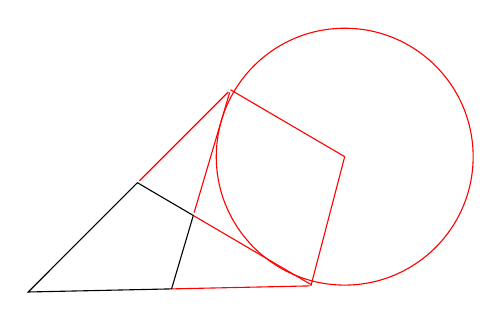
\begin{tikzpicture}[x=1pt,y=1pt]
\draw[red] (155.70,-52.68) -- (123.59,-84.79);
\draw[red] (143.36,-96.27) -- (156.19,-52.88);
\draw[red] (135.23,-123.86) -- (185.05,-122.78);
\draw[red] (185.55,-122.77) -- (197.76,-76.08);
\draw (83.40,-124.98) -- (135.20,-123.86) -- (143.05,-97.34) -- (122.87,-85.50) -- cycle;
\draw[red] (197.76,-76.08) circle (46.41);
\draw[red] (185.57,-122.29) -- (143.14,-97.39);
\draw[red] (197.76,-76.08) -- (156.48,-51.91);
\end{tikzpicture}
\end{document}
